Mit zunehmend signifikanteren Fortschritten im Bereich der Informationstechnologien sind mobile Endger"ate wie Smartphones oder Tablets kaum mehr aus dem Alltag wegzudenken. Mit der Zahl der mobile Devices steigt auch der Bedarf der mobilen Services. Vor allem in der Bankenbranche hat sich in den letzten Jahren der Trend des internet bzw. mobile Banking etabliert und ist in heutigem digitalen Zeitalter zu einem fixem Bestandteil sowohl f"ur Firmen als auch Konsumenten geworden. 

Nach dem Motto: \glqq Customers can use services in wherever they want by location free access and at whenever they want by time free access. \grqq Der Benutzer besitzt alle Freiheiten wo und wann er welche Bankgesch"afte erledigen m"ochte. Insbesondere in S"udkorea, das weltweit zu den f"uhrenden L"andern der wireless Internet Technologien z"ahlt, ist die Anzahl der mobile banking Benutzern drastisch gestiegen. Die Bank of Korea ver"offentlichte quartalsm"a"sig die Daten des nationalen Transaktionsvolumens von internet sowie mobile banking Aktivit"aten.\cite{Jung2011}

\begin{figure}[h!]
	\caption{Anzahl der mobile banking Kunden in S"udkorea 2003-2010}
	\centering
		\includegraphics[scale=1.2]{figures/Jung2011}
\end{figure}

In der Bankbranche ist ein weiteres Innovationsfeld, das eng mit mobile banking verkn"upft ist, das Konzept des contactless payment. Mit dem rasanten Anstieg an mobilen Benutzern ist auch die Nachfrage nach sicherer und bequemer Bezahlung mit Hilfe eines mobilen Ger"ats gestiegen. Der gro"se Wachstum des mobile banking Sektors bietet den unterschiedlichsten Branchen viele M"oglichkeiten von diesem aufstrebenden Markt zu profitieren, inbesondere Mobiltelefonhersteller, Banken und Service Provider. Fr"uher oder sp"ater soll ein einziges mobiles Ger"at die klassische Brieftasche ersetzen. Eine M"oglichkeit des contactless mobile payment basiert auf der Technologie der Near Field Communication (NFC). Viele Mobiltelefone haben heutzutage schon einen NFC Microchip eingebaut, der es erm"oglicht innerhalb von zehn Metern per Funktechnik mit anderen NFC-f"ahigen Ger"aten zu kommunizieren. Somit hat man schon die M"oglichkeit kleine Geldbetr"age "uber Funk zu transferieren um beispielsweise einen Fahrschein mit seinem Smartphone zu kaufen ohne Bargeld oder Bankomat-/Kreditkarte bei sich zu haben. Folgende Abbildung zeigt die Darstellung eines NFC-basierten mobile payment Konzeptes\cite{Kadambi2009}:

\begin{figure}[h!]
	\caption{NFC-basierte mobile payment System}
	\centering
	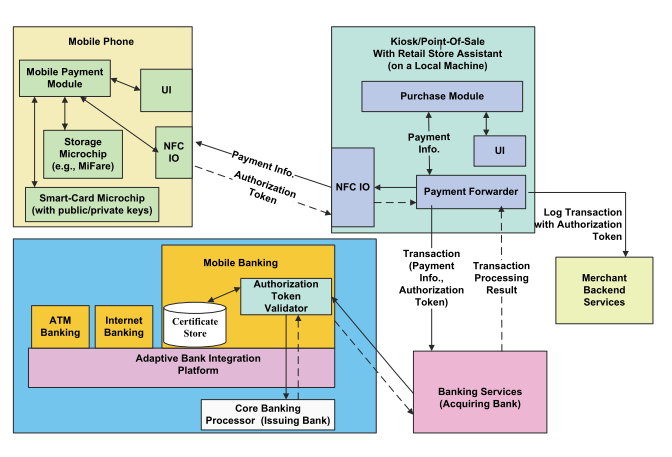
\includegraphics[scale=0.9]{figures/NFCmobilepayment}
\end{figure}